\chapter{Teori}
\label{cha:theory}


%% Vad behöver läsaren veta för att förstå resten av rapporten? %%

\section{Punktmoln}
På senare år har det blivit möjligt att representera objekt i form av ett 3D-representerat punktmoln. Detta har blivit möjligt på grund av utvecklandet av kameror samt laserskannrar. Ett punktmoln är alltså en mängd av punkter i ett tredimensionellt koordinatsystem som representerar ett objekt, se figur \ref{fig:point_cloud_torus}. Punkterna i punktmolnet representerar ofta de yttre kanterna av objektet.

\begin{figure}[H]
	\centering
	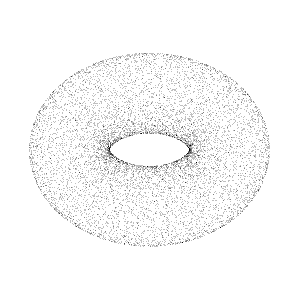
\includegraphics[width=50mm]{figures/Point_cloud_torus.png}
	\caption{Ett punktmoln som representerar ett torus objekt.}
	\label{fig:point_cloud_torus}
\end{figure}


\section{Point Cloud Library}
Point Cloud Library (PCL) är ett bibliotek till C++. PCL presenterar ett avancerat tillvägagångssätt angående ämnet 3D-uppfattning och är tänkt att ge stöd för vanliga 3D-byggstenar som olika applikationer behöver. Biblioteket innehåller algoritmer för:

\begin{itemize}
	\item filtrering
	\item registrering
	\item segmentering
	\item modellanpassning
	\item ytrekonstruering
	\item funktionskalkylering.
\end{itemize}
PCL är alltså ett bibliotek avsett att ge stöd till att behandla punktmolnsdata, iform av olika bearbetningsalgoritmer \cite{rusu20113d}.

Varje algoritm i PCL är definierad via basklasser. Dessa basklasser försöker integrera all vanlig funktionalitet tillsammans med algoritmerna som sedan används igenom hela kedjan i den önskade processen. Detta gör att implementeringen av den aktuella algoritm hålls modulär och tydlig. Den grundläggande kedjan för en önskad process i PCL är som följer:

\begin{itemize}
	\item skapa bearbetningsobjektet (filtrering, registrering, segmentering, etc.)
	\item skicka in det givna punktmolnets data till modulen
	\item ange parametrar
	\item gör beräkningen för att få resultatet.
\end{itemize}
Nedan beskrivs de olika områderna som PCLs algoritmer behandlar \cite{rusu20113d}.

\subsection{Filtrering}
PCLs filtreringsbibliotek innehåller algoritmer för att filtrera ett punktmoln ifrån skräppunkter. Dessa skräppunkter kan uppstå vid skanning av ett objekt eftersom avståndskameran kan reagera på bakgrunden och inte bara på objektet. Det gör att skräppunkter infaller i punkmolnet. Dessa skräppunkter kan filtreras genom att titta på varje punkts grannskap och filtrera ut de som inte uppfyller vissa kriterier. PCLs implementering av filtering är baserad på att beräkna medelavståndet från en punkt till varje granne, för att sedan kolla om detta avstånd ligger inom ett visst intervall. Om inte punkten ligger inom intervallet så filtreras den bort \cite{pcl_filtering}. 
 
\subsection{Segmentering}
PCLs segmenteringsbibliotek innehåller algoritmer för att dela in ett punktmoln i olika kluster. Dessa kluster används för att bryta ner molnet i olika beståndsdelar som kan behandlas oberoende av andra delar. Detta görs ofta för att bearbeta olika eller en specifik del av ett punktmoln. Till exempel kan ett plan segmenteras utifrån en uppsättning av punkter om så önskas \cite{pcl_segmentation}. 
 
\subsection{Modellanpassning}
Modellanpassning i PCL innebär att det finns färdiga metoder och modeller, till exempel plan och cylindrar, som kan kombineras och användas för att upptäcka specifika modeller i ett punktmoln. Detta sub-bibliotek används flitigt av segmenteringsbiblioteket för att upptäcka segment av vanliga geometriska figurer \cite{pcl_model_fitting}.

\subsection{Registrering}
Registrering behandlas ingående av Michael Karlssons utredning, se kapitel \ref{cha:indiv-report-karlsson}.

\subsection{Ytrekonstruering}
PCLs ytrekonstrueringsbibliotek innehåller algoritmer för att rekonstruera de ursprungliga ytorna från 3D-skanningar. Beroende på uppgiften kan PCL till exempel rekonstruera en ojämn yta till en jämn, en meshrepresentation av ett komplett punktmoln eller en yta med normaler \cite{pcl_surface_reconstruction}. 

Att rekonstruera en ojämn yta till en jämn kan vara viktigt om molnet är bullrigt, eller om det består av flera skanningar som inte är perfekt anpassade. PCLs ytrekonstrueringsbibliotek kan även skapa en konkav modell av ett punktmoln. Detta kan vara bra om till exempel gränserna i ett punktmoln behöver extraheras \cite{pcl_surface_reconstruction}.

Att mesha ett punktmoln görs efter att punktmolnen har registreras så de bildar ett komplett punktmoln. Att skapa en meshrepresentation av ett komplett punktmoln innebär att skapa en yta utan punkter. Meshrepresentationen av punktmolnet är alltså en vattentät 3D-modell uppbyggd av polygoner. Den algoritm som används för att mesha ett punktmoln i detta projekt är en trianguleringsalgoritm som körs på ett punktmoln med normaler för att erhålla en yta baserad på grannarna till respektive punkt. För detta krävs alltså ett punktmolnsobjekt som innehåller normalerna till varje punkt i punktmolnet. I detta punktmoln med normaler kan sedan önskade parametrar sättas innan själva trianguleringsalgoritm körs för att generera den önskade meshen \cite{pcl_surface_reconstruction}\cite{pcl_triangulation_algorithm}. 

\subsection{Funktionskalkylering}

\section{3D-skrivare}

%%%%%%%%%%%%%%%%%%%%%%%%%%%%%%%%%%%%%%%%%%%
%			Hur fungerar processen med att skriva ut ett objekt?				%
%			Ifrån 3D-mesh till färdig utskrivet objekt.						%	
%			Martin Lundberg?										%
%%%%%%%%%%%%%%%%%%%%%%%%%%%%%%%%%%%%%%%%%%%

\section{Hållbar utveckling}
Hållbar utveckling är en relevant aspekt i dagens utveckling av programvaror eftersom de används kontinuerligt av samhället. Effekterna som en programvara bidrar med i samhället beror på hur den har producerats och hur den används av konsumenterna. Detta gör att effekterna som en programvara bidrar med i samhället kan vara både positiva men också djupt negativa \cite{raturi2014developing}. Hållbarhet definieras som \textit{förmåga att uthärda} och \textit{bevara funktionen hos ett system under en utsträckt tidsperiod}. Att analysera hållbarhet hos ett mjukvarusystem innebär för de som utvecklar systemet att ha dessa fyra områden i åtanke \cite{lago2015framing}:

\begin{itemize}
	\item Ekonomiskt -  Systemet ska bevara kapital och värde.
	\item Socialt - Systemet ska underhålla samhället.
	\item Miljö - Systemet ska skydda mänskliga välfärden genom att skydda naturens tillgångar.
	\item Tekniskt - Systemet ska utvecklas för att stödja långtidsanvändning.
\end{itemize}

Ett system för 3D-kopiering har många positiva effekter på samhället. Systemet gynnar framförallt miljön eftersom att tillverka en önskad produkt istället för att köpa en fabrikstillverkad sparar avsevärt på naturens tillgångar. Dels kommer 3D-kopieringssystemet att använda mindre energi och dessutom kommer transporterna till och från affären att minska, vilket leder till mindre koldioxidutsläpp. Kreiger \cite{kreiger2013environmental} har gjort en studie där han skriver ut 3D-produkter i plast och jämför kostnaden för att tillverka produkter av plast i en fabrik. Med kostnaden menas den energi som går åt från råmaterial till färdig produkt samt kostnaden som går åt för transport. Det visar sig att tillverka en produkt i en 3D-skrivare kräver mellan 41 till 64 procent mindre energi än att fabrikstillverka produkten. Förklaringen till detta är att produkter som skrivs ut i en 3D-skrivare kan göras mer ihåliga och således kräver de också mindre material. 

Det finns dessutom relaterade studier som visar att det blir billigare att skriva ut en produkt i en 3D-skrivare istället för att köpa en fabrikstillverkad \cite{wittbrodt2013life}. Det här främjar samhället i positiv beaktning eftersom det helt enkelt blir billigare för konsumenter att införskaffa sig de produkter de önskar. 

\subsection{Förbättringspunkter till vårt system}
Vårt system för 3D-kopiering är som tidigare nämnts ett generellt bra system för att främja hållbar utveckling. Det finns däremot en del aspekter som skulle kunna gjorts annorlunda vid systemets uppbyggnad för att ytterligare främja hållbar utveckling. För att utveckla detta har vi valt att titta på hur våra krav framställdes, närmare bestämt besvara dessa frågor:

\begin{itemize}
	\item Hur skulle vi kunna göra annorlunda i kravprocessen?
	\item Vad har vi tagit hänsyn till i kravprocessen?
	\item Hur kan vi bedöma de krav vi satt på systemet med hållbar utveckling i åtanke?
\end{itemize}
Vid framställning av kraven till systemet fanns det inga tankar på att ta fram krav som främjar hållbar utveckling, det på grund av att ingen i projektgruppen hade erfarenheter från hållbar utveckling tidigare och således inte någon tanke på det. Vid framtagning av krav till systemet har alltså ingen hänsyn tagits till att främja hållbar utveckling. Det som har tagits hänsyn till i kravprocessen är endast funktionaliteten av systemet. Att utveckla icke-funktionella krav för att främja denna aspekt är något som vi kunnat gjort annorlunda, det är också ett bra tillvägagångssätt enligt Raturi \cite{raturi2014developing}. 

En förbättring som vi kunde gjort är att systemet ska ha ett icke-funktionellt krav att systemets beräkningar får ta en viss maximal tid. Detta är bra för energi- och miljösynpunkt eftersom hög processoranvändning under en lång tid leder till hög energiförbrukning för systemet. Det finns även en relation mellan hur systemets energianvändning påverkas av hårdvaran i systemet. Den största energianvändande komponenten är processorn och därför skulle systemet även kunna ha ett icke-funktionellt krav att optimera processoranvändningen, detta leder till energianvändningen för systemet minskar vilket är bra ur miljösynpunkt. Enligt Fan, Weber och Barroso \cite{fan2007power} ökar energiförbrukningen linjärt med processoranvändningen, detta är inte helt rättvisande och beror givetvis på vilken processor som används. 

För vårt system innebär det här att vi skulle vilja kombinera dessa två aspekter till ett gemensamt icke-funktionellt krav. En kombination av dessa innebär att vi som grupp skulle behövt göra en studie över hur vi kan optimera processoranvändningen med avseende på energiförbrukning samtidigt som systemet inte får för lång körtid. Det optimala ur energisparningssynpunkt kanske skulle vara att låta systemet använda 70\% av processorn och istället få lite längre körtid. Detta är någonting som vi skulle kunna undersökt i förstudiefasen för senare användning till kravprocessen.

För att bedöma de krav som vi har med hållbar utveckling i åtanke kommer endast de krav som inte har med kärnfunktionaliteten att göra bedömas, eftersom de är nödvändiga för systemets funktionalitet. Andra krav bedöms ur energisynpunkt, om koden är tillräckligt optimerad för att uppfylla kravet eller om det blir för tungt beräkningsmässigt som gör att kravet inte uppfylls. Det skulle även vara möjligt att sätta upp icke-funktionella krav med avseende på det sociala området som gör att användaren känner sig tillfredsställd med produkten och på så vis underhåller samhället. Detta bedöms genom att testa systemet med några användare och se huruvida det uppfyller användarens förväntningar eller inte. 


%%%%%%%%%%%%%%%%%%%%%%%%%%%%%%%%%%%%%%%%%%%%%%%%%%%%%%%%%%%%%%%%%%%%%%
%%% theory.tex ends here
